\documentclass[11pt]{article}

\usepackage[letterpaper,margin=0.85in]{geometry}
\usepackage{amsmath,amssymb,amsfonts}
\usepackage{array,booktabs,longtable,tabularx}
\usepackage{enumitem}
\usepackage{titlesec}
\usepackage{fancyhdr}
\usepackage{lastpage}
\setlength{\headheight}{14pt}
\usepackage{hyperref}
\usepackage{xcolor}
\usepackage{tikz}
\usepackage{caption}
\usetikzlibrary{arrows.meta,positioning,shapes.geometric,calc,fit}

\hypersetup{
  colorlinks=true,
  linkcolor=black,
  urlcolor=black,
  citecolor=black
}

\pagestyle{fancy}
\fancyhf{}
\lhead{Active-Rail Spacetime Metric Engineering Technical Disclosure}
\rhead{Technical Disclosure}
\cfoot{\thepage\ of \pageref{LastPage}}

\titleformat{\section}{\large\bfseries\uppercase}{\thesection.}{0.5em}{}
\titleformat{\subsection}{\normalsize\bfseries}{\thesubsection}{0.5em}{}
\titleformat{\subsubsection}{\normalsize\itshape}{\thesubsubsection}{0.5em}{}
\setlist[itemize]{nosep,leftmargin=1.2em}
\setlist[enumerate]{nosep,leftmargin=1.4em}
\renewcommand{\arraystretch}{1.18}
\setlength{\emergencystretch}{2em}

\newcolumntype{L}[1]{>{\raggedright\arraybackslash}p{#1}}
\newcommand{\dd}{\mathrm{d}}
\newcommand{\sig}{\sigma}
\newcommand{\lp}{\ell_{\mathrm p}}
\newcommand{\rc}{r_{\mathrm c}}

\begin{document}

\begin{center}
{\LARGE \bfseries Active-Rail Spacetime Metric Engineering System}\\[0.35em]
{\Large \bfseries Technical Disclosure and Source-Placement Architecture}\\[0.9em]
{\bfseries Operating Embodiment: One-Space Rail with a Lapse-Staged $2.1c$ Lane}\\[0.8em]
\end{center}

\noindent\textbf{Document purpose.} This document discloses the active-rail metric-service architecture in its one-space operating embodiment: a track of time-staged service fields in a single asymptotically flat space, which carries a protected packet ahead of light through that space and leaves flat space behind each transit. It specifies the metric, the packet choreography, the lapse structure that keeps the demanded tensor admissible, the service sequence, the demanded source and its placement, and the requirements the demand places on physical source families.

\section{Abstract}

An active-rail spacetime metric engineering system is disclosed as a staged transport service in one flat space. A cylindrical service region around the packet's line of travel carries a prescribed shift that moves the packet along the track, enveloped by a convex lapse plateau that rides with the packet. A transverse boundary layer, staged in time with the packet, returns every field to Minkowski values, so the exterior is exactly flat and the standing geometry between transits is flat space. The spatial metric is flat throughout, and the energy density demanded by the geometry is $\rho=-(\partial_r\beta/\alpha)^2/32\pi$: zero where the shift is uniform in radius and lapse-suppressed where it is not. The demanded tensor is therefore a tension without energy, local to the packet and present only during a transit.

In the representative embodiment the packet enters at $0.9c$, crosses a $2.1c$ lane, is caught to $0.95c$ and released, and reaches the track end at exterior time $\sig=3.34$, ahead of light through flat space, which arrives at $\sig=5.0$. The packet stays timelike throughout. The complete demanded tensor is Hawking--Ellis Type I at every evaluated point, under derivative refinement and through the boundary layer into the exterior, with no residual Type IV band. Source units placed along the lane switch on as the packet arrives. The demand's null-energy deficit sets the source requirements: quantum fields supply it at unit lengths below about half a millimetre, Casimir cavities and curvature-coupled scalars supply none, and classical scalars with higher-derivative kinetic terms remain the open family for a rail of macroscopic size.

\section{Technical Field}

The disclosure relates to prescribed spacetime metric engineering, numerical-relativity diagnostics, source-placement architectures, and controlled metric-service systems. More particularly, it relates to a rail-like spacetime metric in one asymptotically flat space in which a time-staged lapse structure envelops a carried shift, a protected packet is carried along a prescribed path, and the demanded source is placed in scheduled units along the route.

\section{Engineering Objective}

A practical spacetime metric engineering architecture benefits from explicit source placement, explicit service timing, and an admissible demanded source. The disclosed system provides a prescribed metric and a source-placement process that:
\begin{enumerate}
\item carries a packet along a track ahead of light through the same flat space, with the packet timelike throughout;
\item keeps the complete demanded tensor Hawking--Ellis Type I, so that a source with a rest frame can supply it;
\item confines the demand to the neighbourhood of the packet and to the duration of each transit, leaving flat space standing;
\item joins every field to an exactly flat exterior within one space, with no change of spatial topology;
\item expresses the service in ADM variables and a demanded-source ledger for placement, timing and acceptance;
\item states the source requirements of the demand in scale-free form, for comparison with candidate source families.
\end{enumerate}

\section{Overview of the Active-Rail System}

The active rail operates as a scheduled metric service in one flat space. Along the track, a cylindrical service region of radius $\rc=1.75$ contains the packet's line of travel. Inside it, spacetime is the exact product of a two-dimensional service metric in $(\sig,z)$ with the flat transverse plane. The service metric carries the packet on a prescribed path through a shift, enveloped by a convex lapse plateau that rises to $e^{4}$ around the packet. Live windows open inside the service domain with the lapse leading the shift and lagging its release.

Around the service region, a transverse boundary layer returns the lapse and shift to Minkowski values by $r=13.25$. A lapse sheath of $e^{1}$ in that layer keeps the stress sign-definite across the shift's radial transition. The sheath rides with the packet on a schedule, so the boundary layer exists only around the packet during a transit, and the geometry before and after each transit is flat space.

The spatial metric is flat everywhere. The shift therefore carries the only energy density, negative and suppressed by the square of the lapse, and the lapse carries stress without energy. The demanded tensor is a tension on the lapse shoulders, local to the packet and present only during a transit. Source units placed along the lane switch on as the packet approaches and off after it passes, each supplying a local, timed stress. A chronology governor schedules service edges on a monotone rail time.

\section{Representative Design Architecture}

The representative design has five coupled layers.
\begin{enumerate}
\item \textbf{Metric-service layer.} The prescribed fields $\alpha$ (clock-lapse) and $\beta$ (carrying flow) on flat spatial slices, with every join infinitely differentiable.
\item \textbf{Packet choreography layer.} A prescribed packet path with entry, acceleration, lane, catch and release; packet windows, rematch sleeve and carry shift centred on the path.
\item \textbf{Lapse layer.} The convex packet lapse plateau of $e^{4}$, live windows gated inside the service domain with lapse lead and release lag, and a plateau with a gentle edge inside an enlarged service domain.
\item \textbf{Boundary layer.} The shift's radial transition, the lapse sheath of $e^{1}$ and the lapse fall to the flat exterior, staged in time with the packet.
\item \textbf{Source layer.} Scheduled source units along the lane, the demanded-source ledger that assigns their duties, and the chronology governor that arms each service edge.
\end{enumerate}

\section{Definitions}

\begin{longtable}{L{0.27\linewidth}L{0.66\linewidth}}
\toprule
\textbf{Term} & \textbf{Meaning in this disclosure} \\
\midrule
Active rail & A spacetime metric service in which scheduled infrastructure fields carry a protected packet along a track. \\
Track & The route along the axis $z$ over which the service fields act, cut off smoothly beyond $|z|=7.5$--$8.5$. \\
Service region & The cylinder $r\le\rc$ around the packet's line of travel, where the service fields take their full values and spacetime is the product of the service metric with the flat transverse plane. It is the packet-safe region of the rail. \\
Transverse boundary layer & The shell $\rc\le r\le13.25$ in which the service fields return to Minkowski values. \\
Service metric & The two-dimensional metric $-\alpha^2\dd\sig^2+(\dd z+\beta\,\dd\sig)^2$ of the service region. \\
Clock-lapse field & The lapse $\alpha$, which sets the local clock rate and the local light speed along the track. \\
Carrying-flow field & The shift $\beta$ along the track, which carries the packet. \\
Packet path & The prescribed worldline $z=\ell_p(\sig)$ of the packet centre, with speed schedule $v(\sig)$. \\
Lane & The interval of the packet path at the lane speed, $2.1c$ in the representative embodiment. \\
Packet lapse plateau & The lapse window around the packet: log-lapse $4$ on a flat top to $|z-\ell_p|\approx1.6$, with convexity $0.3$ along the track and a gentle edge reaching zero at $|z-\ell_p|\approx3.5$. \\
Live windows & The schedules of the carry shift and packet windows, opened inside the service domain from $\sig=-2.4$, with the lapse leading the shift by $1$ and lagging its release by $1.5$. \\
Lapse sheath & A lapse rise of $e^{1}$ across $3.75\le r\le8.75$ in the boundary layer, holding across the shift's radial transition. \\
Time staging & The schedule under which the sheath follows the packet along the track and switches on and off with the transit. \\
Lapse envelope & The condition $\alpha>2r|\partial_z\beta|$ wherever the lapse varies radially under a shift that varies along the track. \\
Static source unit & A source unit at fixed $(z,r,\phi)$. Its frame is the static frame $u\propto\partial_\sig$. \\
Demanded tensor & $T_{ab}=G_{ab}/8\pi$ of the prescribed metric. \\
Demanded-source algebraic gate & The certified Hawking--Ellis classification of the complete demanded tensor on the active metric, under derivative refinement, through the outermost boundary into the exterior, applied before source construction. \\
Null deficit & $d=\max(0,-T(k,k))$ for null $k$ with $u\cdot k=-1$ in a stated frame. \\
Negative-null content & The null deficit integrated over proper volume. \\
C$^\infty$ join rule & Every metric join is infinitely differentiable; polynomial service steps keep their interior profiles and are flattened by an infinitely differentiable step within one tenth of each end. \\
Rail time $T_{\mathrm{rail}}$ & A service-governor chronology variable assigned to a rail or connected rail network. \\
Chronology-governed service sequencing & A service-arming rule in which entry, carry, catch, release, reset and network routing are admitted according to monotone $T_{\mathrm{rail}}$ advance. \\
\bottomrule
\end{longtable}

\section{Representative Metric}

The metric on $(\sig,z,r,\phi)$, with $\phi$ a Killing direction, is
\begin{equation}
\dd s^2=-\alpha^2\dd\sig^2+(\dd z+\beta\,\dd\sig)^2+\dd r^2+r^2\dd\phi^2 ,
\label{eq:metric}
\end{equation}
with $\sig$ the exterior time and $z$ the coordinate along the track. The spatial slices are flat. The fields are
\begin{align}
\log\alpha(\sig,z,r)&=\chi_\alpha(r)\,a(\sig,z)+h(\sig,z)\,E(r),\\
\beta(\sig,z,r)&=\chi_\beta(r)\,b(\sig,z),
\end{align}
where $a$ and $b$ are the service log-lapse and shift along the track, $\chi_\alpha$ and $\chi_\beta$ are radial blends equal to one in the service region, and $h\,E$ is the lapse sheath. The blends are flattened minimum-jerk steps under the C$^\infty$ join rule:
\begin{itemize}
\item $\chi_\beta$ falls from one to zero across $4.25\le r\le6.25$;
\item $\chi_\alpha$ falls from one to zero across $9.25\le r\le13.25$;
\item $E$ rises from zero to one across $3.75\le r\le8.75$ and falls to zero across $9.25\le r\le13.25$.
\end{itemize}
Beyond $r=13.25$ and beyond the service cutoff along the track, the metric is exactly Minkowski.

\subsection{Service region}

For $r\le\rc$ every field is independent of $r$, and the geometry is the product of the service metric with the flat transverse plane. The demanded tensor there has vanishing $(n,z)$ block, and both transverse pressures equal
\begin{equation}
p_r=p_\phi=-\frac{K}{8\pi},
\end{equation}
where $K$ is the Gaussian curvature of the service metric. The along-track null energies vanish identically, and the service-region stress is Type I.

\subsection{Energy density}

With flat slices, the Hamiltonian constraint reads $16\pi\rho=K^2-K_{ij}K^{ij}$, and only the shift bends the slices:
\begin{equation}
K_{\hat z\hat z}=\frac{\partial_z\beta}{\alpha},\qquad K_{\hat z\hat r}=\frac{\partial_r\beta}{2\alpha},
\qquad
\rho=-\frac{1}{32\pi}\left(\frac{\partial_r\beta}{\alpha}\right)^2 .
\end{equation}
The shift's radial transition is the only source of energy density. It is negative and suppressed by the square of the lapse, which exceeds $e^{4}$ across it. Where the shift vanishes, $K_{ij}=0$, and the demanded stress is that of the lapse alone,
\begin{equation}
8\pi T_{ij}=\frac{\delta_{ij}\,D^2\alpha-D_iD_j\alpha}{\alpha},\qquad \rho=0,
\end{equation}
with no energy flux. A lapse that moves or switches in time where the shift vanishes is therefore Type I and carries no energy.

\section{Packet Path and Service Choreography}

The packet follows a prescribed worldline $\ell_p(\sig)$ whose coordinate speed is
\begin{equation}
v(\sig)=v_{\mathrm{in}}+(v_{\mathrm{lane}}-v_{\mathrm{in}})\,\psi\!\left(\frac{\sig-a}{\tau_a}\right)-(v_{\mathrm{lane}}-v_{\mathrm{out}})\,\psi\!\left(\frac{\sig-d}{\tau_d}\right),
\end{equation}
with $\psi$ the rail's smooth step. Every packet-centred field is centred on $\ell_p(\sig)$: the packet windows, the rematch sleeve and the carry shift. At the packet centre the carry shift equals the path speed, so the packet's coordinate speed is the path speed.

\begin{longtable}{L{0.22\linewidth}L{0.71\linewidth}}
\toprule
\textbf{Stage} & \textbf{Setting} \\
\midrule
Entry & $(\sig,z)=(-1.4,-1.4)$ at $0.9c$ \\
Acceleration & to the lane speed over $\Delta\sig=0.3$ \\
Lane & $2.1c$ through the service domain \\
Catch & deceleration to $0.95c$ over $\Delta\sig=0.4$, ending at $z=2.4$; the catch windows span it \\
Release & the live window closes as the packet passes $z=2.6$ \\
Coast & $0.95c$ through flat space to the track end at $z=5$ \\
\bottomrule
\end{longtable}

The release law holds the packet in a matched state, fades the shift through a minimum-jerk profile flattened under the C$^\infty$ join rule, and keeps the lapse active through the handoff. A trailing-edge rematch sleeve, weak at the packet centre and strongest at its trailing edge, softens the local mismatch between the packet speed and the carry shift during catch.

\section{Lapse Plateau, Live Windows and Boundary Layer}

A boundary layer whose lapse rises radially while the shift still varies along the track carries a radial energy flux of about $\partial_z\beta\,\partial_r\log\alpha/8\pi\alpha$, against a null-energy sum that starts from the service region's transverse pressure $-K/8\pi$. The design keeps that sum sign-definite with four elements.
\begin{enumerate}
\item \textbf{Convex packet lapse.} A convexity of $0.3$ in the log-lapse along the track keeps the service region's curvature $K$ negative where the shift varies, so the radial pressure stays positive from the service region outward. Near the packet the convexity changes the lapse by less than $2\%$.
\item \textbf{Packet lapse of $e^{4}$.} The flux at the foot of the sheath falls as $1/\alpha$. At the leading edge of the shift's packet bump, $|\partial_z\beta|$ reaches $8.4$ where the shift meets the rising lapse at $r\approx4.4$--$4.9$, and the lapse envelope there calls for about $74$. The plateau's $e^{4}$ together with the convexity's positive pressure covers it; $e^{3}$ leaves Type IV points.
\item \textbf{Gated live windows.} The windows open inside the service domain, with the rematch shift rising from $\sig=-2.4$, the lapse leading the shift by $1$ and lagging its release by $1.5$. The lapse's own structure along the track meets the shift only on the plateau.
\item \textbf{Lapse sheath of $e^{1}$.} It supplies a positive radial lapse slope across the shift's transition, which keeps the stress in the $(n,z)$ block sign-definite.
\end{enumerate}
The plateau's flat top covers the shift, which reaches about $\pm1.5$ around the packet; a gentle edge brings it to zero by $|z-\ell_p|\approx3.5$, inside a service domain extending to $|z|=7.5$ and cut off by $8.5$.

\subsection{Time staging}

The sheath amplitude is
\begin{equation}
h(\sig,z)=h_0\,T(\sig)\,Z\!\left(z-\ell_p(\sig)\right)\,S(z),
\end{equation}
with $h_0=1$, $Z$ a flat-top window of half-length $2.5$ and edge $1$ that follows the packet, $T$ a schedule switching on over $-4\le\sig\le-3$ and off over $1.5\le\sig\le2.5$, and $S$ the static taper along the track. Wherever the shift vanishes, a lapse that moves or switches in time is Type I and carries no energy, so staging the sheath leaves the demanded tensor admissible. With the sheath staged, the geometry before and after each transit is flat space.

\section{Representative Settings}

\begin{longtable}{L{0.34\linewidth}L{0.59\linewidth}}
\toprule
\textbf{Parameter} & \textbf{Value} \\
\midrule
\endfirsthead
\toprule
\textbf{Parameter} & \textbf{Value} \\
\midrule
\endhead
Spatial metric & flat, $A=1$ everywhere \\
Service-region radius & $\rc=1.75$ \\
Packet path & entry $(-1.4,-1.4)$ at $0.9c$; lane $2.1c$; catch to $0.95c$ ending at $z=2.4$; release at $z=2.6$; track end $z=5$ \\
Packet lapse plateau & log gain $4$; convexity $0.3$; flat top to $|z-\ell_p|\approx1.6$; edge to $3.5$; seventh-order compact window profile \\
Live windows & open inside the service domain from $\sig=-2.4$; lapse lead $1$; release lag $1.5$ \\
Service domain & to $|z|=7.5$, cut off by $8.5$ \\
Shift transition & $4.25\le r\le6.25$ \\
Lapse sheath & $e^{1}$; rise $3.75\le r\le8.75$; fall $9.25\le r\le13.25$; taper along the track beyond $|z|=5.5$ over $1$ \\
Lapse fall & $9.25\le r\le13.25$ \\
Time staging & sheath follows the packet with half-length $2.5$ and edge $1$; schedule on over $[-4,-3]$, off over $[1.5,2.5]$ \\
Exterior & exactly Minkowski beyond $r=13.25$ and beyond the service cutoff \\
Join rule & C$^\infty$ \\
\bottomrule
\end{longtable}

\section{Service Sequence}

The service cycle runs as a literal schedule:
\begin{equation}
\begin{array}{c}
\text{sheath on}\rightarrow\text{live windows open, lapse leading}\rightarrow\text{packet entry}\rightarrow\text{acceleration and lane}\\
\rightarrow\text{catch}\rightarrow\text{release, lapse lagging}\rightarrow\text{sheath off}\rightarrow\text{flat space}.
\end{array}
\end{equation}
The source units along the lane follow the same schedule: each switches on as the packet approaches and off after it passes. Passenger-facing accounting covers entry, lane, catch and release; system accounting covers the whole transit, from $\sig=-8$ to the flat configuration after it.

\section{ADM Translation}

In ADM form the metric of Eq.~\eqref{eq:metric} has lapse $\alpha$, shift $\beta^i=(\beta,0,0)$ along $z$, and flat spatial metric $\gamma_{ij}=\mathrm{diag}(1,1,r^2)$ in $(z,r,\phi)$. The unit normal is
\begin{equation}
n^\mu=\left(\frac{1}{\alpha},-\frac{\beta}{\alpha},0,0\right).
\end{equation}
With $K_{ij}=(D_i\beta_j+D_j\beta_i-\partial_\sig\gamma_{ij})/2\alpha$, the nonvanishing extrinsic curvature is
\begin{equation}
K_{zz}=\frac{\partial_z\beta}{\alpha},\qquad K_{zr}=\frac{\partial_r\beta}{2\alpha},
\end{equation}
so $K=\partial_z\beta/\alpha$ and $K_{ij}K^{ij}=K^2+\tfrac12(\partial_r\beta/\alpha)^2$. The Hamiltonian and momentum constraints give
\begin{equation}
16\pi\rho=K^2-K_{ij}K^{ij}=-\frac12\left(\frac{\partial_r\beta}{\alpha}\right)^2,
\qquad
8\pi j_i=D_jK^j{}_i-D_iK ,
\end{equation}
and the evolution equations give the stresses. The orthonormal demanded tensor is evaluated in the frame $n$, $e_z=\partial_z$, $e_r=\partial_r$, $e_\phi=r^{-1}\partial_\phi$, in which $e_\phi$ is an eigenvector everywhere.

\section{Demanded-Source Algebraic Gate}

Every geometry used for source construction first passes the demanded-source algebraic gate on its active metric, the boundary classification of Le \cite{Le2026}: the certified Hawking--Ellis type of the complete demanded tensor at every sampled point, stable under derivative refinement, through the boundary layer into the exterior. Flux-carrying crossings of the null-energy sums are root-found, and any Type IV band between samples is measured. The lapse envelope is checked at every sample.

\begin{longtable}{L{0.50\linewidth}L{0.20\linewidth}L{0.20\linewidth}}
\toprule
\textbf{Measure} & \textbf{Static sheath} & \textbf{Staged sheath} \\
\midrule
samples ($\sig\in[-8,10]$, $|z|\le10$) & $36{,}381$ & $36{,}381$ \\
non-vacuum boundary-layer points, Type I (Type IV) & $3{,}936{,}637$ ($0$) & $906{,}108$ ($0$) \\
refined: half jet step, 24 nodes per panel & $7{,}891{,}975$ ($0$) & $1{,}815{,}247$ ($0$) \\
resolved flux-carrying crossings (banded) & $4$ ($0$) & $4$ ($0$) \\
lapse envelope violations at the service-region edge & $0$ & $0$ \\
minimum null energy, service region / boundary layer & $-0.26$ / $-0.48$ & $-0.26$ / $-0.47$ \\
exterior & exactly vacuum & exactly vacuum \\
\bottomrule
\end{longtable}

The staged sheath is the operating embodiment; the static sheath is the comparison design with the same service and a standing $e^{1}$ sheath.

\section{Arrival, Packet Safety and Causal Structure}

\subsection{Arrival}

The packet reaches the track end $z=5$ at $\sig=3.34$. Light sent through flat space from the entry event arrives at $\sig=5.0$. The packet therefore leads light through the same flat space by $1.66$, a mean speed of $1.35c$ from entry to track end, and the lead comes entirely from the shift and the lapse.

\subsection{Packet safety}

The packet worldtube is timelike from the approach to the track end. Across the packet body during the live window, the packet moves at most $0.016c$ relative to the local normal observers. Its proper time from $\sig=-8$ to arrival is $294$ against an exterior interval of $11.34$, and its clock runs at most $e^{4}=55$ times exterior time.

\subsection{Service audits}

The audits run on a ledger along the axis over $\sig\in[-8,15]$ and $|z|\le10$ ($52{,}863$ points).
\begin{longtable}{L{0.62\linewidth}L{0.28\linewidth}}
\toprule
\textbf{Audit} & \textbf{Result} \\
\midrule
live packet points (spacelike), maximum norm & $707$ ($0$), $-0.19$ \\
radial escape (escaped/expected, stalled) & $1754/1754$, $0$ \\
entry reachability hits & $0$ \\
centerline probes escaped (maximum norm) & $24/24$ ($-0.0975$) \\
traces entering both-shrinking & $0$ \\
dense-bundle crossings & $0$ \\
bundles below the $0.1$ width criterion (minimum ratio) & $5$ ($0.090$) \\
\bottomrule
\end{longtable}
The five narrow bundles cross the trailing edge of the packet plateau while its lapse switches on; the rays keep their order, and the areal radius along them is constant.

\subsection{Causal structure}

The exterior time $\sig$ is a global time function, since $g^{\sig\sig}=-1/\alpha^2<0$ everywhere, so every causal curve on a single rail advances in $\sig$. With the staged sheath, the standing geometry is flat space, and light through it arrives with light through flat space.

During the lane, the plateau's edges move at $2.1c$ in exterior time. The local light speed along the track passes through the lane speed at the plateau's rear and front edges, and there light along the track moves with the pattern. A ray held at the rear surface shifts in frequency by about $7.4$ e-folds per unit $\sig$ of lane; over one transit the shift reaches $4.5\times10^{9}$. These co-moving light surfaces are a property of every superluminally moving lapse pattern that returns to a flat exterior, and they set a regularity condition on quantum source sectors (Section~\ref{sec:source_families}).

\subsection{Chronology-governed service sequencing}

Operational superluminality brings the standard chronology issue into the service-safety envelope. Everett and Roman showed its network form for Krasnikov tubes: a single directed tube has one-way superluminal behaviour, while a pair of tubes can form a time machine \cite{EverettRoman1997}. Shoshany and Snodgrass give a two-warp construction in which linked warp geometries form a closed timelike geodesic \cite{ShoshanySnodgrass2024}. The active rail treats this as a safety-engineering problem for service arming, reset timing and network routing.

Let $T_{\mathrm{rail}}$ be the chronology variable of a rail or connected rail network. A permitted service edge $A\rightarrow B$ satisfies
\begin{equation}
T_{\mathrm{rail}}(B_{\mathrm{arrive}})\ge T_{\mathrm{rail}}(A_{\mathrm{depart}})+\Delta_{\mathrm{safety}},
\end{equation}
where $\Delta_{\mathrm{safety}}$ covers staging, catch and release recovery, clock uncertainty, relative-motion margin and routing margin. A multi-leg cycle $C$ is admitted when
\begin{equation}
\sum_{e\in C}\Delta T_{\mathrm{rail}}(e)>\Delta_{\mathrm{cycle}} .
\end{equation}
A connected network shares one chronology governor or a certified translation into one global ordering. Two rails in relative motion can close causal curves, as two Krasnikov tubes can; the governor admits their service edges only in a common monotone order.

\section{Demand and Source Placement}

\subsection{Demand}

\begin{longtable}{L{0.62\linewidth}L{0.28\linewidth}}
\toprule
\textbf{Measure} & \textbf{Staged sheath} \\
\midrule
standing energy, each sign & $0$ \\
standing negative-null content & $0$ \\
transit: peak negative energy, instantaneous & $1.9\times10^{-4}$ \\
transit: peak negative-null content, instantaneous & $141$ \\
transit: negative-null content integrated over $\sig$ & $799$ \\
peak stress component & $2.9$ \\
source speed relative to static source units, maximum & $0.23c$ \\
\bottomrule
\end{longtable}

Positive energy vanishes throughout. The demand exists for $\sig\in[-3.9,2.8]$, local to the packet. Its negative-null content lies in the lapse's outer falls ($456$ of $799$), the sheath rise ($255$), and the inner band, sheath plateau and service region. The null condition fails along $r$ on $5.2\%$ of the transit's proper volume, along $z$ on $4.7\%$ and along $\phi$ on $2.2\%$. No point satisfies the dominant energy condition.

In the frame of the static source units, the null deficit peaks at $0.48$ where the outer falls begin, near the track end as the packet coasts, and reaches $0.26$ inside the service region during the carry. Static source units exist at every point throughout the transit, and their proper time runs up to $256$ times $\sig$.

\subsection{Physical scale}

The shape of the demand is fixed, and its magnitude scales with the rail's unit length $L$: stresses as $1/L^2$ and integrated contents as $L$. Both are set by the packet's neighbourhood and are independent of route length.

\begin{longtable}{L{0.62\linewidth}L{0.28\linewidth}}
\toprule
\textbf{Measure} & \textbf{Value} \\
\midrule
peak negative energy, $L=1$ m & $2.5\times10^{23}$ kg \\
peak negative-null content, $L=1$ m, as mass & $1.9\times10^{29}$ kg, $0.095\,M_\odot$ \\
peak stress, $L=1$ m & $3.5\times10^{44}$ Pa \\
peak stress, $L=1$ km & $3.5\times10^{38}$ Pa \\
\bottomrule
\end{longtable}

\subsection{Source-placement ledger}

\begin{longtable}{L{0.24\linewidth}L{0.45\linewidth}L{0.22\linewidth}}
\toprule
\textbf{Source role} & \textbf{Demand and placement} & \textbf{Primary diagnostic} \\
\midrule
Service-region pressure & Transverse pressure $-K/8\pi$ with zero energy density and zero pressure along the track, in the packet's path during the carry & $K$, service-region null deficit \\
Shift transition & Lapse-suppressed negative energy $-(\partial_r\beta/\alpha)^2/32\pi$ across $4.25\le r\le6.25$ while the shift is live & $\rho$, flux, lapse envelope \\
Sheath rise & Stress without energy on the rising lapse; null deficit on its shoulder & null deficit, principal pressures \\
Outer falls & Stress without energy where the lapse returns to one; the largest share of the negative-null content & null deficit, radial null energy \\
Scheduled units & Mechanically independent source modules (C1) at fixed positions along the lane, switched on as the packet approaches and off after it passes; the stress pattern moves at up to $0.23c$ relative to them & static-frame demand history \\
\bottomrule
\end{longtable}

\section{Source-Family Requirements}
\label{sec:source_families}

The null deficit lies in the outer falls, the sheath rise, the inner band and the service region during each transit, and it sets the requirement on physical sources. Ordinary matter and fields that respect the null energy condition supply the remainder of the tensor. The following requirements hold for the representative embodiment.

\subsection{Quantum fields}

For a massless scalar along an inertial worldline with 4-velocity $u$, the sampled null energy obeys \cite{FewsterRoman2003}
\begin{equation}
\int\langle T_{ab}k^ak^b\rangle\,g(\tau)^2\,\dd\tau\;\ge\;-\frac{(u\cdot k)^2}{12\pi^2}\int g''(\tau)^2\,\dd\tau ,
\end{equation}
which for a Gaussian $g^2$ of standard deviation $\tau_0$ is $-(u\cdot k)^2/64\pi^2\tau_0^4$. With $\tau_0$ a fraction $f$ of the local curvature radius and inverse acceleration along the static source units' worldlines, the demand requires
\begin{equation}
N\;\ge\;Q\left(\frac{L}{\lp}\right)^2
\end{equation}
free fields, with $Q=0.013$ at $f=0.1$ and $3\times10^{-6}$ at $f=0.01$. The governing requirement comes from broad, gentle deficits in the outer falls and at the switch-on of the sheath and live windows. At the recorded normalization, one unit equal to $204\,\lp$, the requirement is about $560$ fields; at $L=1$ m it is $5\times10^{67}$.

$N$ light fields bring gravity to strong coupling at the species length $\ell_*\approx\sqrt N\,\lp$ \cite{Dvali2010}, which here equals $\sqrt Q\,L=0.12\,L$ at $f=0.1$, the demand's sharpest curvature radius. A quantum-sourced rail therefore operates at the gravitational cutoff of its own field content, at every scale. With Newtonian gravity verified to $52\,\mu$m \cite{Lee2020}, quantum fields supply the rail at unit lengths up to about $0.45$ mm ($2.9$ cm at $f=0.01$). A quantum source sector also stays regular across the co-moving light surfaces of each lane, where the renormalized stress of superluminal warp geometries grows exponentially with the lane's duration \cite{FinazziLiberatiBarcelo2009}.

\subsection{Casimir cavities}

An ideal-mirror cavity of gap $a$ has null deficit $\pi^2\hbar c/180a^4$ along its normal, and it matches the demand at $a=0.58\sqrt{\lp L}$: $2.3\times10^{-18}$ m at $L=1$ m, with modes at $530$ GeV. The thinnest electron plasma mirror that reflects those modes carries about $10^{7}$ times the deficit it bounds, in both the non-relativistic and the ultra-relativistic regimes of its electrons. Casimir cavities supply no net deficit at any scale.

\subsection{Curvature-coupled classical fields}

A scalar coupled to curvature through $F(\phi)R$, with a healthy kinetic term and NEC-respecting matter, satisfies
\begin{equation}
F''\le8\pi T(k,k)\,F
\end{equation}
along every affinely parametrized null geodesic, where $F>0$ keeps the effective gravitational coupling positive and finite. Any positive $F$ that is constant at the ray's entry is bounded by the zero-energy solution of $-\dd^2/\dd\lambda^2+8\pi T(k,k)$, and vanishes where that solution does. Every radial ray through the packet during the carry, and every ray launched at the sixteen deepest deficits in its minimizing direction, carries a bound state of that operator: $F$ reaches zero at the inner edge of the outer falls, $r\approx10.65$, where the effective coupling diverges. The criterion is independent of scale, in agreement with the classical wormhole results \cite{BarceloVisser2000,Butcher2015} and with the averaged null energy condition obeyed by curvature-coupled scalars within effective field theory \cite{FlissFreivogelKontouPardoSantos2024}.

\subsection{Classical fields with higher-derivative kinetic terms}

Scalar theories whose action contains second derivatives of the field (kinetic gravity braiding, Galileons, beyond-Horndeski theories) violate the null energy condition classically without ghosts on suitable backgrounds \cite{DeffayetPujolasSawickiVikman2010,Rubakov2014}. Beyond-Horndeski theories admit wormholes free of ghost and gradient instabilities \cite{FrancioliniHuiPencoSantoniTrincherini2019}, which Horndeski theories exclude \cite{EvseevMelichev2018}, and perturbations about null-energy-violating backgrounds in these theories generally propagate superluminally \cite{DubovskyGregoireNicolisRattazzi2006}. Their supply is classical and scales with the demand as $1/L^2$. This family is the source family for a rail of macroscopic size; its construction specifies the action, supplies the deficit in the outer falls and the sheath rise during each transit, and establishes the stability of its perturbations on the time-dependent background.

\section{Relation to the Wormhole--Warp Correspondence}

The metric of Eq.~\eqref{eq:metric} has flat spatial slices and a shift along the track: it is the Nat\'ario--Alcubierre warp form \cite{Alcubierre1994,Natario2002} with a non-unit lapse, on the warp side of the wormhole--warp-drive correspondence of Garattini and Zatrimaylov \cite{GarattiniZatrimaylov2024}. The rail's distinctive elements relative to a warp bubble are the prescribed packet path inside a service region, the lapse plateau that envelops the carried shift, the time-staged boundary layer that leaves flat space standing, and the scheduled source units along the route. Clark, Hiscock and Larson studied null geodesics of the Alcubierre spacetime and found horizon-like access structures for superluminal operation \cite{ClarkHiscockLarson1999,MullerWeiskopf2012}; the rail's co-moving light surfaces at the plateau's edges are the corresponding structure, and the service audits evaluate the packet, escape and bundle behaviour around them.

\section{Diagnostic Architecture and Acceptance Path}

\subsection{Reusable diagnostic layers}

\begin{enumerate}
\item Exact field builder for $\alpha$ and $\beta$ on the axial metric, with second-order jets in $(\sig,z,r)$.
\item Generated orthonormal Einstein tensor of the axial metric, checked against an independent finite-difference kernel and against the Riemann tensor assembled from the jets.
\item Certified Hawking--Ellis classifier with degenerate-spectrum resolution, band root-finding at flux-carrying crossings, derivative refinement and exterior checks.
\item Near-packet design screen with packet-resolved offsets.
\item Demand census by zone and energy-condition class, in coordinate and proper measures, with source velocities relative to normal and static observers.
\item Packet path ledger, packet clock and path-aware service audits: live packet norm, radial escape, entry reachability, scheduled probes, trace expansion and dense bundles.
\item Static-frame demand histories along source-unit worldlines, with curvature radius and acceleration.
\item Quantum-inequality requirement with self-consistent Gaussian windows, screened over every worldline and sampled explicitly on leading worldlines with a fixed null direction.
\item Null-geodesic tracer with the zero-energy solution of $-\dd^2/\dd\lambda^2+8\pi T(k,k)$ from both ends and the null-energy integral.
\item Casimir cavity and plasma-mirror bounds.
\end{enumerate}

\subsection{Acceptance standard}

A prescribed metric is accepted for source construction when:
\begin{enumerate}
\item the complete demanded tensor is certified Hawking--Ellis Type I at every evaluated point of the active metric, under derivative refinement and through the boundary layer into an exactly flat exterior;
\item every flux-carrying crossing resolves without a Type IV band;
\item every metric join is infinitely differentiable;
\item the packet worldtube is timelike from approach to arrival;
\item the service audits find complete radial escape, no entry reachability hits, no traces entering both-shrinking regions and no dense-bundle crossings;
\item the packet reaches the track end ahead of light through the same flat space;
\item the demand is recorded by zone, energy-condition class and frame, with its source-family requirements stated in scale-free form;
\item the chronology governor maps every service edge into monotone rail-time advance.
\end{enumerate}
The representative embodiment meets each of these criteria. Physical load-bearing acceptance additionally supplies the component tensors of the source sectors, their exchange and recoil accounting, and their coupled dynamics.

\section{Engineering Acceptance Criteria}

\begin{longtable}{L{0.27\linewidth}L{0.47\linewidth}L{0.18\linewidth}}
\toprule
\textbf{Criterion} & \textbf{Meaning} & \textbf{Status} \\
\midrule
Algebraic admissibility & Type I demanded tensor at every evaluated point, refined, with no resolved band & met \\
Exterior & exactly Minkowski beyond the boundary layer and the service cutoff & met \\
Standing geometry & flat space between transits & met (staged) \\
Packet safety & timelike packet worldtube; clock rate at most $55$ times exterior time & met \\
Arrival & track end reached $1.66$ ahead of light through flat space & met \\
Service audits & escape, reachability, traces and bundles & met \\
Demand locality & demand confined to the packet's neighbourhood for $\sig\in[-3.9,2.8]$ & met \\
Source-family requirement & a source family that supplies the null deficit at the target scale & open: higher-derivative classical scalars; quantum fields below $0.45$ mm \\
Finite source assembly & C1 units with counted tensors, exchange and recoil on the shared geometry & open \\
Coupled dynamics & preparation, back-reaction, stability of the lapse maximum and recovery & open \\
\bottomrule
\end{longtable}

\section{Risk Controls and Diagnostic Controls}

\begin{enumerate}
\item \textbf{Boundary-layer flux.} Radial energy flux where the lapse rises under a shift that varies along the track is controlled by the convex packet lapse, the $e^{4}$ plateau, the gated live windows and the lapse sheath.
\item \textbf{Thin packet-edge bands.} Type IV edges at the packet's leading boundary are controlled by the convexity of the plateau and resolved by packet-offset screens at spacing $0.02$.
\item \textbf{Plateau-cutoff stress.} Stress concentration where the plateau meets the service cutoff is controlled by the gentle plateau edge inside the enlarged service domain.
\item \textbf{Join regularity.} Curvature growth at metric joins is controlled by the C$^\infty$ join rule.
\item \textbf{Standing demand.} Demand between transits is removed by staging the sheath with the packet.
\item \textbf{Packet clock.} The packet's clock rate is set by the lapse envelope at the sharpest along-track gradient of the shift's packet bump; a smoother bump lowers it.
\item \textbf{Co-moving light surfaces.} Frequency shifts at the plateau's edges during the lane are recorded by the null-geodesic tracer and bounded by the lane's duration.
\item \textbf{Chronology.} Service arming is controlled by the rail-time governor across single-rail and connected-network operation.
\end{enumerate}

\section{Illustrative System Diagram}

\begin{center}
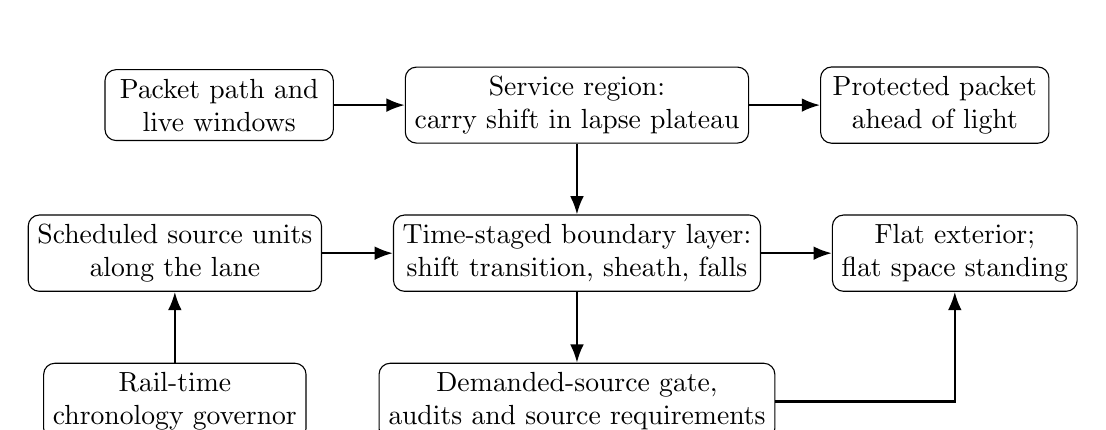
\begin{tikzpicture}[
  node distance=0.9cm,
  block/.style={draw, rounded corners, align=center, minimum height=0.85cm, minimum width=2.9cm},
  arrow/.style={-Latex, thick}
]
\node[block] (path) {Packet path and\\live windows};
\node[block, right=of path] (region) {Service region:\\carry shift in lapse plateau};
\node[block, right=of region] (packet) {Protected packet\\ahead of light};
\node[block, below=of region] (layer) {Time-staged boundary layer:\\shift transition, sheath, falls};
\node[block, left=of layer] (units) {Scheduled source units\\along the lane};
\node[block, right=of layer] (exterior) {Flat exterior;\\flat space standing};
\node[block, below=of layer] (gate) {Demanded-source gate,\\audits and source requirements};
\node[block, below=of units] (governor) {Rail-time\\chronology governor};
\draw[arrow] (path) -- (region);
\draw[arrow] (region) -- (packet);
\draw[arrow] (region) -- (layer);
\draw[arrow] (layer) -- (exterior);
\draw[arrow] (units) -- (layer);
\draw[arrow] (layer) -- (gate);
\draw[arrow] (governor) -- (units);
\draw[arrow] (gate.east) -| (exterior.south);
\end{tikzpicture}
\end{center}

\section{Claim-Oriented Embodiments}

The following claim-oriented embodiments clarify the technical scope of the disclosure.

\begin{enumerate}
\item A method of operating a prescribed spacetime metric service in one asymptotically flat space, comprising defining a track, carrying a packet along a prescribed path through a service region around the track with a shift, enveloping the shift in a lapse plateau around the packet, and returning the lapse and shift to Minkowski values across a transverse boundary layer.

\item The method of item 1, wherein the spatial metric is flat and the demanded energy density is $-(\partial_r\beta/\alpha)^2/32\pi$.

\item The method of item 1, wherein the service region is the product of a two-dimensional service metric with the flat transverse plane, and its demanded stress is a transverse pressure $-K/8\pi$ with $K$ the Gaussian curvature of the service metric.

\item The method of item 1, wherein the packet path comprises entry, acceleration to a lane speed above the speed of light in the exterior, a catch to a coasting speed below it, and release, and wherein the packet windows, rematch sleeve and carry shift are centred on the path.

\item The method of item 4, wherein the packet reaches the track end ahead of light through the same flat space while its worldtube remains timelike.

\item The method of item 1, wherein the lapse plateau is convex along the track, so that the Gaussian curvature of the service metric stays negative where the shift varies.

\item The method of item 1, wherein live windows open inside the service domain with the lapse leading the shift and lagging its release.

\item The method of item 1, wherein the boundary layer comprises a shift transition on a rising lapse, a lapse sheath holding across that transition, and a lapse fall to the exterior value, arranged so that the lapse envelope $\alpha>2r|\partial_z\beta|$ holds wherever the lapse varies radially.

\item The method of item 8, wherein the lapse sheath follows the packet along the track and switches on and off with the transit, so that the standing geometry between transits is flat space.

\item The method of item 1, wherein every metric join is infinitely differentiable, with polynomial service steps flattened by an infinitely differentiable step near their ends.

\item The method of item 1, further comprising classifying the complete demanded tensor of the active metric with a certified Hawking--Ellis eigensystem under derivative refinement and through the boundary layer into the exterior, root-finding every flux-carrying crossing, and accepting a geometry whose demanded tensor is Type I at every evaluated point.

\item A spacetime metric engineering system comprising a service region carrying a shift enveloped by a lapse plateau, a transverse boundary layer with a time-staged lapse sheath, an exactly flat exterior, and source units placed along the track and scheduled to switch on as a packet approaches and off after it passes.

\item The system of item 12, wherein the demanded tensor is a tension without energy on the lapse shoulders, present only during a transit and local to the packet.

\item The system of item 12, further comprising a demanded-source ledger that assigns the service-region pressure, the shift transition, the sheath rise and the outer falls to source roles, with source velocities recorded relative to the static source units.

\item A source-evaluation process comprising computing the demanded tensor of a prescribed rail metric in the frame of static source units, recording the null-deficit history along their worldlines with the curvature radius and acceleration, and computing the number of quantum fields required by a quantum inequality with self-consistent sampling windows.

\item The process of item 15, further comprising tracing null geodesics through the demand, computing the zero-energy solution of $-\dd^2/\dd\lambda^2+8\pi T(k,k)$ from each end, and recording where a curvature coupling $F(\phi)R$ reaches zero.

\item The process of item 15, further comprising comparing the demand's null deficit with Casimir cavities, including the energy of the mirrors that bound them.

\item The method of item 1, further comprising a rail-time chronology governor in which each armed service edge, reset interval and network link advances a common rail time with safety margin.
\end{enumerate}

\section{Diagnostic Data Products}

\begin{enumerate}
\item the \href{supporting_reports/AXIAL_TRACK.md}{axial track}: construction of the one-space metric, generated kernel and independent checks;
\item the \href{supporting_reports/ONE_SPACE_REVISION.md}{one-space revision}: lapse envelope, shear identity and staged boundary layers;
\item the \href{supporting_reports/CHOREOGRAPHY_PASS.md}{choreography pass}: packet path, lane speeds, arrival and gate;
\item the \href{supporting_reports/DEMAND_CENSUS.md}{demand census}: demand by zone, class and frame;
\item the \href{supporting_reports/AMPLITUDE_PASS.md}{amplitude pass}: flat support and minimum pre-sheath;
\item the \href{supporting_reports/LAPSE_AND_STAGING_PASS.md}{lapse and staging pass}: the operating embodiment, its gate, demand, packet clock and audits;
\item the \href{supporting_reports/SOURCE_SCALING_TEST.md}{source scaling test}: static-frame demand, quantum-inequality requirement, Casimir bounds and the null-geodesic test for curvature-coupled fields;
\item the \href{supporting_reports/THROAT_GEOMETRY_CLARIFICATION.md}{geometry clarification}: the relation of the one-space rail to the earlier spherical throat metric.
\end{enumerate}

\section{Conclusion}

The active rail organizes spacetime metric engineering as a scheduled service in one flat space. A prescribed shift carries the packet along a path inside a service region, a convex lapse plateau envelops the shift, and a boundary layer staged with the packet returns every field to an exactly flat exterior. The spatial metric is flat, so the lapse carries stress without energy and the shift carries only a lapse-suppressed negative energy. The demanded tensor is Type I everywhere, local to the packet and present only during a transit, and the packet reaches the track end ahead of light through the same flat space while remaining timelike.

The demand's null deficit defines the source requirement. Quantum fields supply it at sub-millimetre unit lengths, where the rail operates at the gravitational cutoff of its field content. Casimir cavities and curvature-coupled scalars supply none. Classical scalars with higher-derivative kinetic terms carry a classical supply that scales with the demand, and they form the source family for a macroscopic rail. Source units along the lane, scheduled with the transit and coordinated by the rail-time governor, place that supply where and when the demand requires it.

\section{Source Code and Artifact Repository}

The version-controlled source code, supporting reports, disclosure source, and project history are maintained at
\href{https://github.com/dgoldman0/spacetime-metric-engineering}{https://github.com/dgoldman0/spacetime-metric-engineering}.
The revision of this disclosure describing the earlier spherical throat metric is preserved at the commit
\begin{center}
\href{https://github.com/dgoldman0/spacetime-metric-engineering/tree/2146526c7a70691cd1ac1f8f4928b99d7cca0c19}{\texttt{2146526c7a70691cd1ac1f8f4928b99d7cca0c19}}.
\end{center}
Large generated run-data artifacts are regenerated by the scripts named in each report.

\begin{thebibliography}{99}

\bibitem{Alcubierre1994}
M. Alcubierre,
\textit{The Warp Drive: Hyper-Fast Travel within General Relativity},
Class. Quantum Grav. 11, L73--L77, 1994.
arXiv:gr-qc/0009013.

\bibitem{Natario2002}
J. Nat\'ario,
\textit{Warp Drive with Zero Expansion},
Class. Quantum Grav. 19, 1157--1165, 2002.
arXiv:gr-qc/0110086.

\bibitem{GarattiniZatrimaylov2024}
R. Garattini and K. Zatrimaylov,
\textit{On the Wormhole--Warp Drive Correspondence},
JCAP 08 (2024) 061.
arXiv:2401.15136.

\bibitem{Le2026}
A. T. Le,
\textit{On the Boundary Cost of Source-Consistent Warp Shells},
arXiv:2605.25417, 2026.

\bibitem{ClarkHiscockLarson1999}
C. Clark, W. A. Hiscock, and S. L. Larson,
\textit{Null Geodesics in the Alcubierre Warp Drive Spacetime: The View from the Bridge},
Class. Quantum Grav. 16, 3965--3972, 1999.
arXiv:gr-qc/9907019.

\bibitem{MullerWeiskopf2012}
T. M{\"u}ller and D. Weiskopf,
\textit{Detailed Study of Null and Time-Like Geodesics in the Alcubierre Warp Spacetime},
Gen. Relativ. Gravit. 44, 509--533, 2012.
arXiv:1107.5650.

\bibitem{EverettRoman1997}
A. E. Everett and T. A. Roman,
\textit{Superluminal Subway: The Krasnikov Tube},
Phys. Rev. D 56, 2100--2108, 1997.
arXiv:gr-qc/9702049.

\bibitem{ShoshanySnodgrass2024}
B. Shoshany and B. Snodgrass,
\textit{Warp Drives and Closed Timelike Curves},
Class. Quantum Grav. 41, 205005, 2024.
arXiv:2309.10072.

\bibitem{FewsterRoman2003}
C. J. Fewster and T. A. Roman,
\textit{Null Energy Conditions in Quantum Field Theory},
Phys. Rev. D 67, 044003, 2003.
arXiv:gr-qc/0209036.

\bibitem{Dvali2010}
G. Dvali,
\textit{Black Holes and Large N Species Solution to the Hierarchy Problem},
Fortsch. Phys. 58, 528--536, 2010.
arXiv:0706.2050.

\bibitem{Lee2020}
J. G. Lee, E. G. Adelberger, T. S. Cook, S. M. Fleischer, and B. R. Heckel,
\textit{New Test of the Gravitational $1/r^2$ Law at Separations down to 52 $\mu$m},
Phys. Rev. Lett. 124, 101101, 2020.

\bibitem{FinazziLiberatiBarcelo2009}
S. Finazzi, S. Liberati, and C. Barcel\'o,
\textit{Semiclassical Instability of Dynamical Warp Drives},
Phys. Rev. D 79, 124017, 2009.
arXiv:0904.0141.

\bibitem{BarceloVisser2000}
C. Barcel\'o and M. Visser,
\textit{Scalar Fields, Energy Conditions, and Traversable Wormholes},
Class. Quantum Grav. 17, 3843--3864, 2000.
arXiv:gr-qc/0003025.

\bibitem{Butcher2015}
L. M. Butcher,
\textit{Traversable Wormholes and Classical Scalar Fields},
Phys. Rev. D 91, 124031, 2015.
arXiv:1503.04145.

\bibitem{FlissFreivogelKontouPardoSantos2024}
J. R. Fliss, B. Freivogel, E.-A. Kontou, and D. Pardo Santos,
\textit{Non-Minimal Coupling, Negative Null Energy, and Effective Field Theory},
SciPost Phys. 16, 119, 2024.
arXiv:2309.10848.

\bibitem{DeffayetPujolasSawickiVikman2010}
C. Deffayet, O. Pujol\`as, I. Sawicki, and A. Vikman,
\textit{Imperfect Dark Energy from Kinetic Gravity Braiding},
JCAP 10 (2010) 026.
arXiv:1008.0048.

\bibitem{Rubakov2014}
V. A. Rubakov,
\textit{The Null Energy Condition and Its Violation},
Phys. Usp. 57, 128--142, 2014.
arXiv:1401.4024.

\bibitem{EvseevMelichev2018}
O. A. Evseev and O. I. Melichev,
\textit{No Static Spherically Symmetric Wormholes in Horndeski Theory},
Phys. Rev. D 97, 124040, 2018.

\bibitem{FrancioliniHuiPencoSantoniTrincherini2019}
G. Franciolini, L. Hui, R. Penco, L. Santoni, and E. Trincherini,
\textit{Stable Wormholes in Scalar-Tensor Theories},
JHEP 01 (2019) 221.

\bibitem{DubovskyGregoireNicolisRattazzi2006}
S. Dubovsky, T. Gr\'egoire, A. Nicolis, and R. Rattazzi,
\textit{Null Energy Condition and Superluminal Propagation},
JHEP 03 (2006) 025.

\end{thebibliography}

\end{document}
